\documentclass[notes,slidesec,a4]{seminar}
\usepackage[spanish]{babel}
\usepackage[utf8]{inputenc}

\usepackage{t-gsyc-6}
\usepackage{fancybox}
\usepackage{graphics}
\usepackage{moreverb}
\usepackage{alltt}
\usepackage{html}
\usepackage{hthtml}
\usepackage{amsmath}
\usepackage[normalsize]{subfigure}
\usepackage{url}
\usepackage{listings}

\usepackage{eurosym}

\title{VisualHFSM 5.0}
\author{Samuel Rey Escudero}

\cop{Samuel Rey Escudero}
\address{samuel.rey.escudero@gmail.com}

\begin{document}
\maketitle

%%--------------------------------------------------------------

\begin{hslide}
\slsect{Índice}
\begin{itemize}
\item Introducción 
\item Objetivos
\item Infraestructura
\item Desarrollo
\item Conclusiones
\end{itemize}
\end{hslide}

%%--------------------------------------------------------------

\begin{hslide}
\slsect{Introducción}

\begin{minipage}{5cm}
\begin{center}
\begin{itemize}
\item {\bf Visión por computador}
\item Sensores RGBD
\item Seguimiento de personas y sensores RGBD en el Grupo de Robótica
\end{itemize}
\end{center}
\end{minipage} \hfill


\begin{minipage}{5cm}
\begin{center}
\begin{figure}
\includegraphics[height=1.8cm]{img/dyson2}
\includegraphics[height=1.8cm]{img/deteccion_cuerpo}
\hspace{0.6cm}
\includegraphics[width=3cm]{img/camscanner}
\end{figure}
\end{center}
\end{minipage}

\end{hslide}

%%--------------------------------------------------------------

\begin{hslide}
\begin{minipage}{6cm}
\begin{center}
\begin{itemize}
\item Visión por computador
\item {\bf Sensores RGBD}
\item Seguimiento de personas y sensores RGBD en el Grupo de Robótica
\end{itemize}
\begin{figure}
\includegraphics[height=1.5cm]{img/xtion}
\end{figure}
\end{center}
\end{minipage} \hfill
\begin{minipage}{5cm}
\begin{center}
\begin{figure}
\includegraphics[height=3.2cm]{img/kinect}
\vspace{0.2cm}
\includegraphics[height=2.6cm]{img/kinect2}
\end{figure}
\end{center}
\end{minipage}
\end{hslide}

%%--------------------------------------------------------------    

\begin{hslide}
\begin{minipage}{6cm}
\begin{center}
\begin{itemize}
\item Visión por computador
\item Sensores RGBD
\item {\bf Seguimiento de personas y sensores RGBD en el Grupo de Robótica}
\end{itemize}
\end{center}
\end{minipage} \hfill
\begin{minipage}{5cm}
\begin{center}
\begin{figure}
\includegraphics[width=4cm]{img/frivas}
\includegraphics[width=3.5cm]{img/jnavarro}
\end{figure}
\end{center}
\end{minipage}
\end{hslide}

%%--------------------------------------------------------------  

\begin{hslide}
\slsect{Objetivos}
Diseñar y programar un prototipo funcional con un algoritmo capaz de detectar y contar personas a partir de la información de sensores RGBD.
\begin{itemize}
\item Extracción de primer plano
\item Detección de \textit{blobs}
\item Seguimiento de personas
\end{itemize}
\end{hslide}

%%---------------------------------------------------------------

\begin{hslide}
\slsect{Infraestructura}
\begin{minipage}{6cm}
\begin{center}
\begin{itemize}
\item Sensor RGBD
\item JdeRobot 5.2
\item GNU/Linux - Ubuntu 14.04
\item Lenguaje de programación C++
\item Librerías: Point Cloud, OpenCV, cvBlob, Qt
\item Herramienta Make
\item Subversion
\end{itemize}
\end{center}
\end{minipage} \hfill
\begin{minipage}{5cm}
\begin{center}
\begin{figure}
\includegraphics[height=3cm]{img/opencv}
\end{figure}
\end{center}
\end{minipage}
\end{hslide}

%%---------------------------------------------------------------

\begin{hslide}
\slsect{Diseño y Desarrollo}
\begin{center}
\begin{figure}
\includegraphics[width=11cm]{img/caja_negra}
\end{figure}
\end{center}
\end{hslide}

%%---------------------------------------------------------------

\begin{hslide}
\slsubsect{Diagrama de bloques}
\begin{itemize}
\item Captura de información desde sensor RGBD
\item Extracción de primer plano
\item Detección de \textit{blobs} de interés
\item Seguimiento y conteo de \textit{blobs}
\end{itemize}

\begin{center}
\begin{figure}
\includegraphics[width=10cm]{img/diagrama}
\end{figure}
\end{center}
\end{hslide}

%%---------------------------------------------------------------

\begin{hslide}
\slsubsect{Extracción de primer plano}
En el primer plano se encuentran las personas, por eso nos quedamos con el primer plano para filtrar los píxeles que no son de interés. Para ello utilizamos la imagen de profundidad y obtenemos una imagen binarizada.\par
Dos modos de extracción de primer plano:
\begin{itemize}
\item Mezcla de gaussianas
\begin{figure}
\begin{center}
	\includegraphics[height=2.5cm]{img/imagen_rgb_gauss}
	\includegraphics[height=2.5cm]{img/imagen_depth_gauss}
	\includegraphics[height=2.5cm]{img/MOG}
\end{center}
\end{figure}
\end{itemize}
\end{hslide}

%%---------------------------------------------------------------

\begin{hslide}\footnotesize
\begin{lstlisting}
//Umbralizamos la imagen de distancia
threshold(rgb[0], result, 0, 255, 
	CV_THRESH_BINARY|CV_THRESH_OTSU);

//Extraccion de primer plano por mezcla de gaussianas
pMOG= new cv::BackgroundSubtractorMOG2();
blur(result, result, cv::Size(4,4));
pMOG->operator()(result, result);

//Erosionamos la imagen para eliminar el ruido
cv::Mat kernel= cv::getStructuringElement(cv::MORPH_RECT,
	cv::Size(7,7), cv::Point(3,3));
	morphologyEx(result, result, CV_MOP_CLOSE, kernel);
\end{lstlisting}\normalsize
\end{hslide}

%%---------------------------------------------------------------

\begin{hslide}
\begin{itemize}
\item Diferencia de imágenes sobre fondo fijo
\begin{figure}
\begin{center}
	\includegraphics[height=3cm]{img/esquema_diferencia}
\end{center}
\end{figure}

\begin{figure}
\begin{center}
	\includegraphics[height=2.5cm]{img/original}
	\includegraphics[height=2.5cm]{img/fondo_aprendido}
	\includegraphics[height=2.5cm]{img/diferencia}
\end{center}
\end{figure}
\end{itemize}
\end{hslide}

%%---------------------------------------------------------------

\begin{hslide}\footnotesize
\begin{lstlisting}
//Restamos la imagen de distancia del sensor RGBD
//y la imagen de fondo aprendido
absdiff(rgb_first[0], rgb_depth[0], result);
    
//Umbralizamos la imagen y erosionamos
//para eliminar el ruido
threshold(result, result, 0, 255, 
	CV_THRESH_BINARY|CV_THRESH_OTSU);
cv::Mat kernel = cv::getStructuringElement
	(cv::MORPH_ELLIPSE, cv::Size(4,4));
morphologyEx(result, result, cv::MORPH_CLOSE, kernel);
\end{lstlisting}\normalsize
\end{hslide}

%%---------------------------------------------------------------

\begin{hslide}
\slsubsect{Segmentación de imágenes}
A partir de la imagen de primer plano obtenida, agrupamos los píxeles que forman parte del mismo objeto o persona.Dos modos:
\begin{itemize}
\item Segmentación mediante librería cvBlob
\begin{figure}
\begin{center}
	\includegraphics[height=2.5cm]{img/imagen_rgb}
	\includegraphics[height=2.5cm]{img/imagen_depth}
	\includegraphics[height=2.5cm]{img/cvblobs}
\end{center}
\end{figure}
\end{itemize}
\end{hslide}

%%---------------------------------------------------------------

\begin{hslide}\footnotesize
\begin{lstlisting}
// Convertimos  a IplImage y a escala de grises
IplImage *gray = cvCreateImage(cvGetSize(&img), 
	IPL_DEPTH_8U, 1);
cvCvtColor( &img, gray, CV_BGR2GRAY );

// Obtenemos los blobs y los representamos en la imagen
IplImage *labelImg = cvCreateImage(cvGetSize(gray), 
	IPL_DEPTH_LABEL, 1);
CvBlobs blobs;
unsigned int result = cvLabel(gray, labelImg, blobs);
cvRenderBlobs(labelImg, blobs, &img, &img);

// Convertimos de nuevo a cv::Mat
cv::Mat out(&img);
\end{lstlisting}\normalsize
\end{hslide}

%%---------------------------------------------------------------

\begin{hslide}
\begin{itemize}
\item Segmentación mediante \textit{watershed}
\begin{figure}
\begin{center}
	\includegraphics[height=2.5cm]{img/imagen_original_watershed}
	\includegraphics[height=2.5cm]{img/imagen_depth_watershed}
	\includegraphics[height=2.5cm]{img/imagen_watershed}
\end{center}
\end{figure}
\end{itemize}
\end{hslide}

%%---------------------------------------------------------------

\begin{hslide}\footnotesize
\begin{lstlisting}
// Encontramos las semillas
std::vector<std::vector<cv::Point> > contours;
findContours(sub_depth_gray, contours, CV_RETR_EXTERNAL,
	CV_CHAIN_APPROX_SIMPLE);

// Identificamos los objetos de la imagen
ncomp = contours.size();
cv::Mat markers = cv::Mat::zeros(dist.size(), CV_32SC1);
for (int i = 0; i < ncomp; i++)
        drawContours(markers, contours, i, 
        	cv::Scalar::all(i+1), -1);
watershed(img, markers);
\end{lstlisting}\normalsize
\end{hslide}

%%---------------------------------------------------------------

\begin{hslide}
Otras técnicas de segmentación de objetos:
\begin{itemize}
\item Algoritmo K-medias
\item Métodos basados en el histograma
\item Método de detección de bordes
\item Método de crecimiento de semillas
\item Método basado en modelos
\end{itemize}
\end{hslide}

%%---------------------------------------------------------------

\begin{hslide}
\slsubsect{Seguimiento visual de objetos}
El seguimiento utilizando cvBlob se basa en el seguir el mismo objeto en fotogramas consecutivos a lo largo del tiempo, asociando \textit{blobs} a las personas que se están siguiendo en ese instante (\textit{tracks})
\begin{itemize}
\item Decide por cercanía y tamaño del \textit{blob}
\item Utiliza matriz de adyacencias: muy eficiente
\end{itemize}
\begin{figure}
\begin{center}
	\includegraphics[height=1.5cm]{img/matriz_cvblob}
\end{center}
\end{figure}
\end{hslide}

%%---------------------------------------------------------------

\begin{hslide}
\slsubsect{Interfaz gráfico}
GUI programado con la librería Qt:
\begin{itemize}
\item Imágenes de tipo cv::Mat utilizando canvas de Qt
\item Panel de opciones utilizando \textit{widgets} QCheckBox
\end{itemize}
\begin{figure}
\begin{center}
	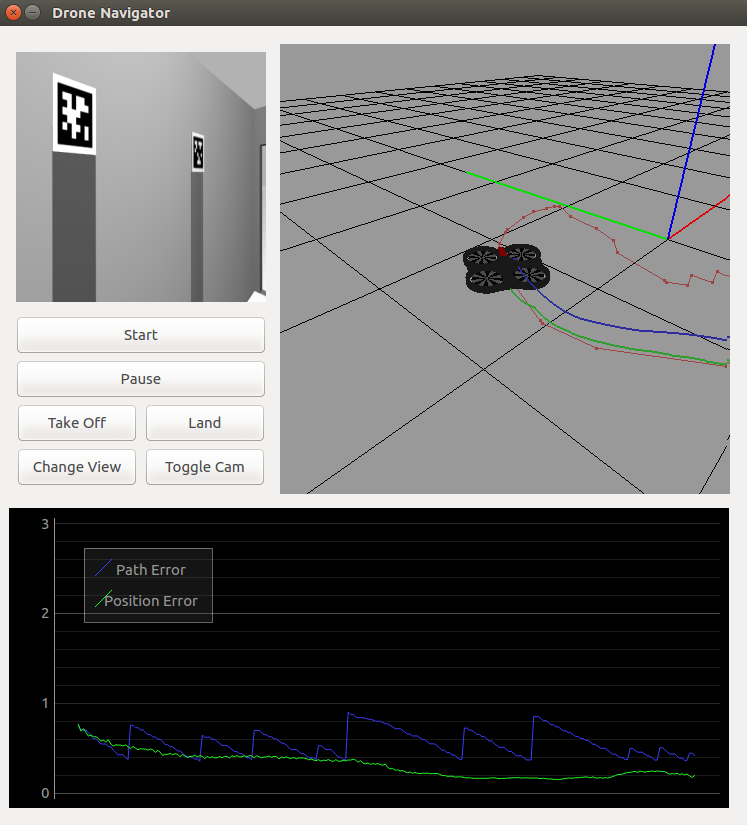
\includegraphics[height=4cm]{img/gui}
\end{center}
\end{figure}
\end{hslide}

%%---------------------------------------------------------------

\begin{hslide}
\begin{itemize}
\item Nube de puntos en visor 3D utilizando qvtkWidget, esto nos permite observar la escena 3D desde cualquier ángulo moviéndolo con el ratón.
\end{itemize}
\begin{figure}
\begin{center}
	\includegraphics[height=2.5cm]{img/3d1}
	\includegraphics[height=2.5cm]{img/3d2}
	\includegraphics[height=2.5cm]{img/3d3}
\end{center}
\end{figure}
\end{hslide}

%%---------------------------------------------------------------

\begin{hslide}
\slsect{Experimentos}
\slsubsect{Ejecución típica con cvLabel y mezcla de gaussianas}
\begin{center}
\begin{figure}
	\includegraphics[height=2.5cm]{img/ex1a_rgb}
	\includegraphics[height=2.5cm]{img/ex1a_depth}
	\includegraphics[height=2.5cm]{img/ex1a_blob}
\end{figure}
\end{center}
\end{hslide}

%%---------------------------------------------------------------

\begin{hslide}
\slsubsect{Experimentos sobre extracción de primer plano}
Diferencia de imágenes con fondo fijo
\begin{center}
\begin{figure}
	\includegraphics[height=2cm]{img/ex2b_rgb}
	\includegraphics[height=2cm]{img/ex2b_depth}
	\includegraphics[height=2cm]{img/ex2b_diff1}
\end{figure}
\end{center}
\textbf{Mezcla de gaussianas}
\begin{center}
\begin{figure}
	\includegraphics[height=2cm]{img/ex2a_rgb}
	\includegraphics[height=2cm]{img/ex2a_depth}
	\includegraphics[height=2cm]{img/ex2a_gauss}
\end{figure}
\end{center}
\end{hslide}

%%---------------------------------------------------------------

\begin{hslide}
\slsubsect{Experimentos sobre segmentación}
Segmentación mediante \textit{watershed}
\begin{center}
\begin{figure}
	\includegraphics[height=2cm]{img/ex2d_rgb}
	\includegraphics[height=2cm]{img/ex2d_depth}
	\includegraphics[height=2cm]{img/ex2d_water1}
\end{figure}
\end{center}
\textbf{Segmentación mediante cvLabel}
\begin{center}
\begin{figure}
	\includegraphics[height=2cm]{img/ex2f_rgb}
	\includegraphics[height=2cm]{img/ex2f_depth}
	\includegraphics[height=2cm]{img/ex2f_blob}
\end{figure}
\end{center}
\end{hslide}

%%---------------------------------------------------------------

\begin{hslide}
\slsect{Conclusiones}
\begin{itemize}
\item Se ha programado un prototipo funcional capaz de detectar y contar personas (1000 LOC)
\item Cumple criterios de tiempo real y estructura modular
\item Se han realizado experimentos para validar el algoritmo y cada una de sus partes
\begin{itemize}
\item Extracción de primer plano: mezcla de guassianas y fondo fijo
\item Segmentación: cvBlob y watershed
\item Seguimiento: cvBlob
\end{itemize}
\end{itemize}
\end{hslide}

%%---------------------------------------------------------------

\begin{hslide}
\slsubsect{Trabajos futuros}
\begin{itemize}
\item Minimizar la intervención del usuario en el procesamiento de vídeos
\item Seguimiento directamente en 3D
\end{itemize}
\end{hslide}

%%---------------------------------------------------------------

\end{document}